%!TEX root = ../thesis.tex

\section{学習フェーズ}
提案手法で用いる学習フェーズのシステムを\figref{Fig:suggest_learning_sys}に示す. 自律移動を行う地図を用いたルールベース制御器から目標方向を生成し, データセットに加えている. 
なお, 厳密にはルールベース制御を構成するwaypoint\_navにより目標方向を生成している. 
提案手法では, 
% \figref{Fig:overview}に示すように
LiDARとオドメトリを入力とする地図を用いたルールベース制御器による自律移動を, カメラ画像と目標方向を用いて模倣学習する.

% \vspace{3cm}
\begin{figure}[hbtp]
     \centering
    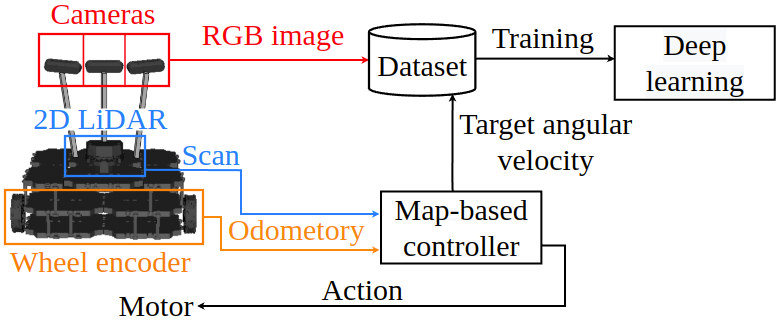
\includegraphics[keepaspectratio, scale=0.45]
         {images/conventional.png}
    \caption{Learning phase system of conventional method}
    \label{Fig:conventional}
   \end{figure}   

\begin{figure}[hbtp]
  \centering
 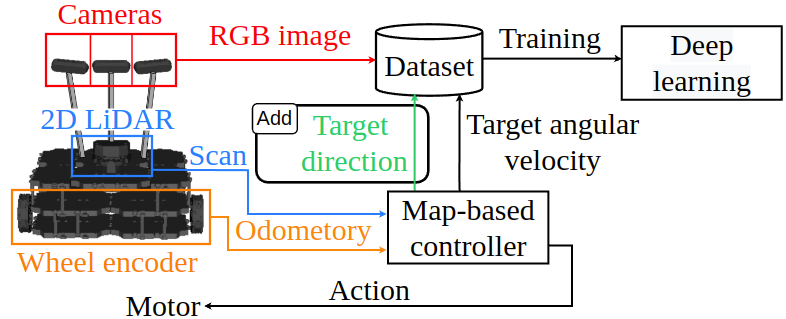
\includegraphics[keepaspectratio, scale=0.45]
      {images/suggest_learning_sys2.png}
 \caption{Learning phase system of proposed method}
 \label{Fig:suggest_learning_sys}
\end{figure}

% \begin{figure}[hbtp]
%   \centering
%  \includegraphics[keepaspectratio, scale=0.6]
%       {images/overview.png}
%  \caption{Overview learning phase}
%  \label{Fig:overview}
% \end{figure}

% \subsubsection{etc...}
\newpage
